%------------------------------------------------------------------------------
\documentclass[A4,11pt]{article}
%\documentclass[letterpaper,11pt]{article} %For use in US
\usepackage{latexsym}
\usepackage[empty]{fullpage}
\usepackage{titlesec}
\usepackage{marvosym}
\usepackage[usenames,dvipsnames]{color}
\usepackage{verbatim}
\usepackage{enumitem}
\usepackage[hidelinks]{hyperref}
\usepackage[english]{babel}
\usepackage{tabularx}
\usepackage{tikz}
\input{glyphtounicode}
\usepackage{booktabs}
\usepackage{palatino}

\usepackage{multicol} % Add this package to your preamble


%--------LOGO------------
\newcommand*{\GoogleScholarlogosymbol}{
\includegraphics[height=.7\baselineskip]{GSlogo}}
\newcommand*{\ResearchGatelogosymbol}{
\includegraphics[height=.7\baselineskip]{RGlogo}}
\newcommand*{\Scopuslogosymbol}{
\includegraphics[height=.7\baselineskip]{SClogo}}
\newcommand*{\ORCIDlogosymbol}{
\includegraphics[height=.7\baselineskip]{ORCIDlogo}}


%-----PAGE SETUP---------------------------------------------------------------
% Adjust margins
\addtolength{\oddsidemargin}{-1cm}
\addtolength{\evensidemargin}{-1cm}
\addtolength{\textwidth}{2cm}
\addtolength{\topmargin}{-1cm}
\addtolength{\textheight}{2cm}

\urlstyle{same}

\raggedbottom
\raggedright
\setlength{\tabcolsep}{0cm}

%---------Sections formatting------------------------
\titleformat{\section}{
  \vspace{-4pt}\scshape\raggedright\large
}{}{0em}{}[\color{black}\titlerule \vspace{-5pt}]

% Ensure that .pdf is machine readable/ATS parsable
\pdfgentounicode=1

%-----CUSTOM COMMANDS FOR FORMATTING SECTIONS----------------------------------
\newcommand{\CVItem}[1]{
  \item\small{
    {#1 \vspace{-2pt}}
  }
}

\newcommand{\CVSubheading}[4]{
  \vspace{-2pt}\item
    \begin{tabular*}{0.97\textwidth}[t]{l@{\extracolsep{\fill}}r}
      \textbf{#1} & #2 \\
      \small#3 & \small #4 \\
    \end{tabular*}\vspace{-7pt}
}

\newcommand{\CVSubSubheading}[2]{
    \item
    \begin{tabular*}{0.97\textwidth}{l@{\extracolsep{\fill}}r}
      \text{\small#1} & \text{\small #2} \\
    \end{tabular*}\vspace{-7pt}
}

\newcommand{\CVSubItem}[1]{\CVItem{#1}\vspace{-4pt}}

\renewcommand\labelitemii{$\vcenter{\hbox{\tiny$\bullet$}}$}

\newcommand{\CVSubHeadingListStart}{\begin{itemize}[leftmargin=0.5cm, label={}]}
% \newcommand{\resumeSubHeadingListStart}{\begin{itemize}[leftmargin=0.15in, label={}]} % Uncomment for US
\newcommand{\CVSubHeadingListEnd}{\end{itemize}}
\newcommand{\CVItemListStart}{\begin{itemize}}
\newcommand{\CVItemListEnd}{\end{itemize}\vspace{-5pt}}


%------------------------------------------------------------------------------
% CV STARTS HERE  %
%------------------------------------------------------------------------------
\begin{document}

%\begin{center} \Huge
%	\underline{\bf Curriculum vitae}
%\end{center}
%-----HEADING------------------------------------------------------------------
\begin{minipage}[c]{0.05\textwidth}
\-\
\end{minipage}
\begin{minipage}[c]{0.2\textwidth}
\begin{tikzpicture}
    \clip (0,0) circle (1.75cm);
    \node at (0,-.7) {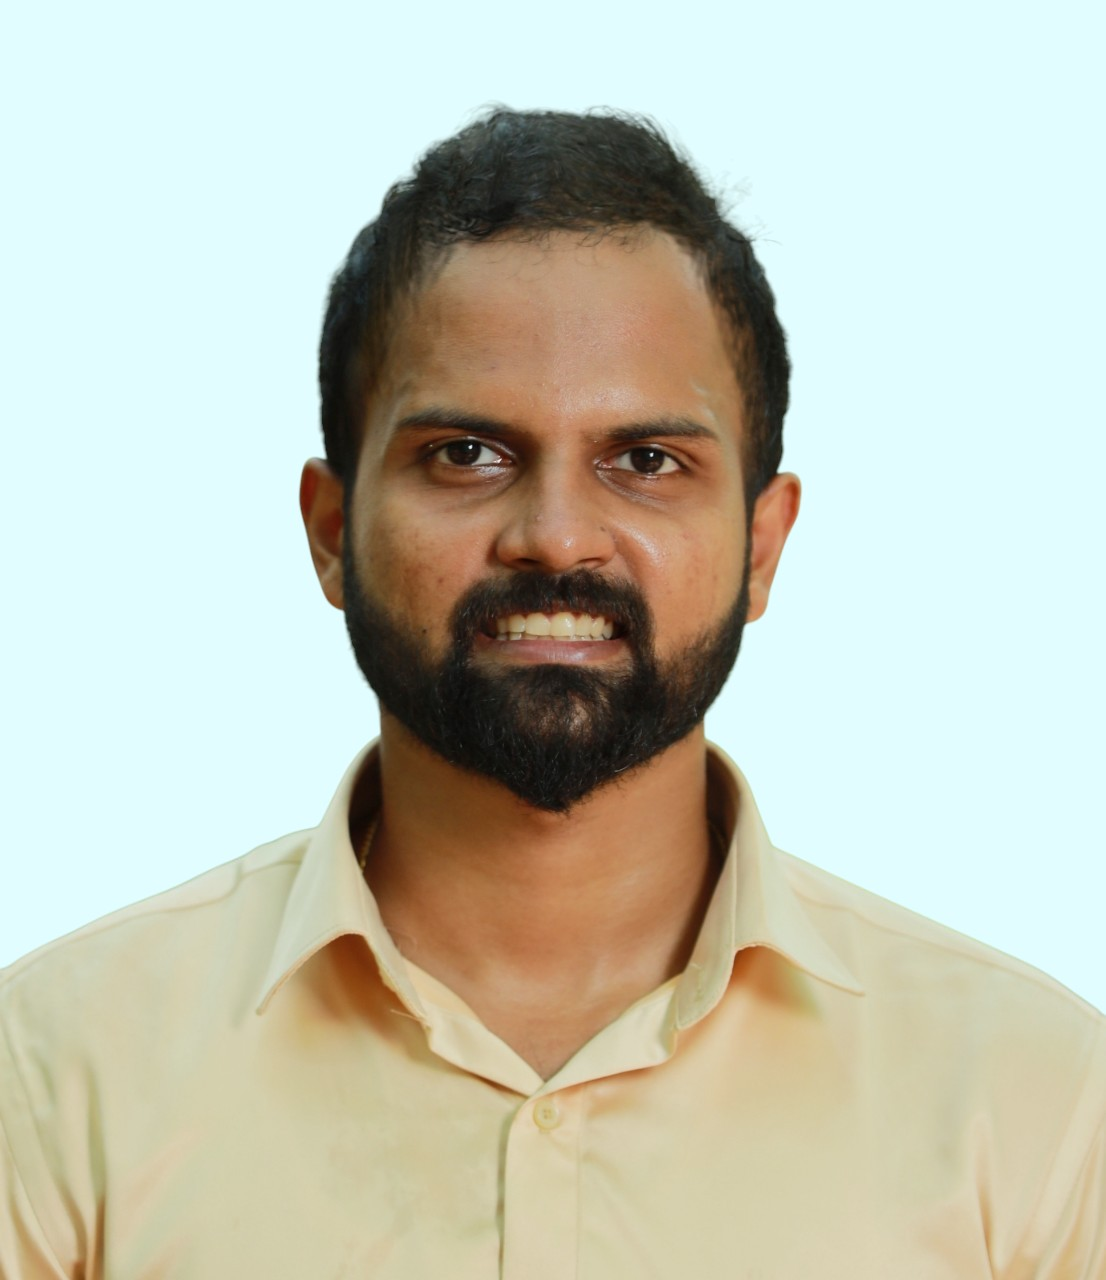
\includegraphics[width = 5cm]{myphoto}}; 
    % if necessary the picture may be moved by changing the at (coordinates)
    % width defines the 'zoom' of the picture
\end{tikzpicture}
\hfill\vline\hfill
\end{minipage}
\begin{minipage}[c]{0.4\textwidth}
    \textbf{\huge \scshape{Manoj Nagappan}} \\ \vspace{1pt} 
    \small{PhD Research Scholar} \\
    \small{SRM Institute of Science and Technology} \\
    \small{Tamil Nadu, India} \\
    % \Mobilefone\ \small{+91\,75\,58\,13\,22\,32} \\
    \vspace{0.2cm}
    \MVAt\  \href{mailto:manojnu04@gmail.com}{\underline{manojnu04@gmail.com}}\\
    \ORCIDlogosymbol\ \ \href{https://orcid.org/0009-0005-7220-1287}{\underline{https://orcid.org/0009-0005-7220-1287}}\\
    \Scopuslogosymbol\ \ \href{https://www.scopus.com/authid/detail.uri?authorId=57836199000}{\underline{https://www.scopus.com/authid/detail.uri?authorId=57836199000}}\\
    \GoogleScholarlogosymbol\ \ \href{https://scholar.google.com/citations?hl=en&authuser=2&user=NWYlZ10AAAAJ}{\underline{scholar.google.com/citations?hl=en\&authuser=2\&user=NWYlZ10AAAAJ}}\\
    \ResearchGatelogosymbol\ \ \href{https://www.researchgate.net/profile/Manoj-Nagappan}{\underline{https://www.researchgate.net/profile/Manoj-Nagappan}}\\
\end{minipage}

% \vspace{0.5cm}
%-----EDUCATION----------------------------------------------------------------
\section{\textbf{\huge Education}}
\begin{table}[h]
\centering
\begin{tabular}{||c|c|c|c|c|c||}
\toprule
\ \ \textbf{Course} \ \ & \ \ \textbf{Institution} \ \ & \ \ \textbf{University/} \ \ &\ \ \textbf{Year} \  \ & \ \ \textbf{Class} \  \ &\  \ \textbf{Medium} \\
  &  & \ \ \textbf{Board} \ \ & \ \ \textbf{of Passing} \ \ & \ \ \textbf{and CGPA} \ \ & \ \ \textbf{of Instruction} \ \ \\
\midrule\midrule
\ \ \textbf{Doctor } \ \ & \ \ SRM \ \ & \ \  & \ \ Expected to \ \ & \ \ - \ \ & \ \ English \ \ \\
\ \ \textbf{of} \ \ & \ \ Institute of Science \ \ & \ \  \ \ & graduate in  & \ \  \ \ &  \\
\ \ \textbf{Philosophy} \ \ & \ \  and Technology, \ \ & \ \  - \ \ & 2027  & \ \  \ \ &  \\
\ \textbf{(Mathematics)} \ & \ \ Chengalpattu, \ \ & \ \  \ \ &   &  &  \\
& \ \ Tamil Nadu, India \ \ & \ \  \ \ &   &  &  \\
\midrule
 \ \ \textbf{Master } \ \ & \ \ Nesamony \ \ & \ \ Manonmaniam & \ \ 2022 \ \ & \ \ First class \ \ & \ \ English \ \ \\
 \ \ \textbf{of} \ \ & \ \ Memorial \ \ & \ \ Sundaranar \ \ &   & \ \ with distinction \ \ &  \\
 \ \ \textbf{Science} \ \ & \ \ Christian College, \ \ & \ \ University, \ \ &   & \ \ (CGPA: {\bf 9.73/10}) \ \ &  \\
 \ \textbf{(Mathematics)} \ & \ \ Kanniyakumari, \ \ & \ \ Tirunelveli, \ \ &   &  &  \\
  & \ \ Tamil Nadu, India \ \ & \ \ Tamil Nadu, India \ \ &   &  &  \\
\midrule
\ \ \textbf{Bachelor } \ \ & \ \ Lekshmipuram \ \ & \ \ Manonmaniam & \ \ 2020 \ \ & \ \ First class \ \ & \ \ English \ \ \\
\ \ \textbf{of} \ \ & \ \ College of \ \ & \ \ Sundaranar \ \ &   & \ \ with distinction \ \ &  \\
\ \ \textbf{Science} \ \ & \ \ Arts \& Science, \ \ & \ \ University, \ \ &   & \ \ (CGPA: {\bf 8.66/10}) \ \ &  \\
\ \textbf{(Mathematics)} \ & \ \ Kanniyakumari, \ \ & \ \ Tirunelveli, \ \ &   &  &  \\
& \ \ Tamil Nadu, India \ \ & \ \ Tamil Nadu, India \ \ &   &  &  \\
\bottomrule
\end{tabular}
\end{table}

% \vspace{1cm}
%-----Interests-------------------------------------------------------------------
\section{\textbf{\huge Current Research Interests}}
\begin{multicols}{2}
	\begin{itemize}
		\item Robotics
		\item Teleoperation
		\item Reinforcement Learning
		\item Control Theory
	\end{itemize}
\end{multicols}

% \newpage

%-----WORK EXPERIENCE----------------------------------------------------------
\section{\textbf{\huge Experience}}
\textbf{Research Experience}
\begin{itemize}
	\item \textbf{TEEP Research Intern (Jul 2026 -- Present)}
	\begin{itemize}
		\item[] \underline{Research focus}: \textit{\textbf{Bilateral teleoperation of robotic manipulators}}
		\item[] \underline{Institute}: \textit{\textbf{National Taiwan Normal University, Taipei, Taiwan}}
		\item[] \underline{Department}: \textit{\textbf{Electrical Engineering}}
		\item[] \underline{Lab}: \textit{\textbf{Educational Robotics Center (ERC)}}
		\item[] \underline{Supervisor}: \textit{\textbf{Prof. Saeed Saeedvand}}
		\item[] \underline{Work}:
		\begin{itemize}
			\item Developing a bilateral leader--follower teleoperation system using \textbf{ROS~2 Control}.
			\item Implementing joint-level control in \textbf{MIT mode} (PD + feedforward torque control).
			\item Implementing \textbf{gravity compensation} based on the robot's dynamic model.
			\item Designing robot parts in \textbf{SolidWorks} and generating \textbf{URDF} models for simulation and control.
			\item Mechanical assembly of the robot hardware and electrical wiring of the actuators and power system.
		\end{itemize}
	\end{itemize}
	\item \textbf{Project Associate - I (Mar 2024 -- May 2025)}
	\begin{itemize}
		\item[] \underline{Project title}: \textit{\textbf{Design and Analysis of fractional-order Clifford-valued neural networks and its application to image encryption}}
		\item[] \underline{Project funded by}: \textit{\textbf{Science and Engineering Research Board (SERB), Department of Science and Technology, Government of India}} 
		\item[] \underline{Grand file number:} \textit{\textbf{EEQ/2023/000513}}
		\item[] \underline{Institute}: \textit{\textbf{SRM Institute of Science and Technology, Chengalpattu, Tamil Nadu, India}}
		\item[] \underline{Department}: \textit{\textbf{Mathematics}}
		\item[] \underline{Principal investigator}: \textit{\textbf{Dr. R. Sriraman}, Assistant professor, Division of Mathematics, Vellore Institute of Technology, Chennai, Tamil Nadu, India}
		\item[] \underline{Work}:
		\begin{itemize}
			\item Theoretical analysis of fractional-order Clifford-valued systems.
			\item Implemented image encryption and decryption schemes in \textbf{MATLAB}.
		\end{itemize}
	\end{itemize}
\end{itemize}
\textbf{Teaching Experience}
\begin{itemize}
	\item \textbf{Assistant Professor (Jul 2023 -- Feb 2024)}
	\begin{itemize}
		\item[] \underline{Institute}: \textit{\textbf{Sri Vidya Mandir Arts \& Science college, Krishnagiri, Tamil Nadu, India}}
		\item[] \underline{Department}: \textit{\textbf{Mathematics}}
	\end{itemize}
\end{itemize}

%-----AWARDS AND HONORS----------------------------------------------------------
%\section{\textbf{\huge 
%Awards and Honors}}
%\begin{itemize}
%	\item
%	\end{itemize}

%-----MEMBERSHIP----------------------------------------------------------
\section{\textbf{\huge 
		Membership in Academic Bodies}}
\begin{itemize}
	\item Graduate Student Member (2025-2026) - Institute of Electrical and Electronics Engineers (IEEE).
\end{itemize}

%-----RESEARCH PUBLICATIONS----------------------------------------------------
\section{\textbf{\huge Research Publications}}
 \textbf{Published Papers in SCI/SCIE (Peer-reviewed)}
\begin{itemize}
	\item[2026] {\bf N. Manoj}, R. Sriraman, \lq\lq Relaxed synchronization analysis of fractional-order Clifford-valued delayed neural networks via novel inner product-based inequality'', \textbf{\textit{Physica Scripta (IF: 2.6)}}, vol. 101, Article No. 425202.
	\textit{\url{https://doi.org/10.1088/1402-4896/aeb198}}
	\item[2026] {\bf N. Manoj}, R. Sriraman, \lq\lq Projective synchronization of fractional-order BAM Clifford-valued delayed memristive neural networks: An inner product-based inequality'', \textbf{\textit{Mathematical Methods in the Applied Sciences (IF: 2.0)}}.\\ \textit{\url{https://doi.org/10.1002/mma.70592}}
	\item[2026] R. Sriraman, {\bf N. Manoj}, \lq\lq Finite-time stabilization of fractional-order fuzzy Clifford-valued neural networks using novel inequalities'', \textbf{\textit{Physica Scripta (IF: 2.6)}}, vol. 101, Article No. 265206.
	\textit{\url{https://doi.org/10.1088/1402-4896/ae8133}}
	\item[2026] R. Sriraman, {\bf N. Manoj}, \lq\lq Finite-time Stability of fractional-order delayed Clifford-valued neural networks via a novel non-separation approach'', \textbf{\textit{Computational and Applied Mathematics (IF: 2.3)}} , vol. 45, Article No. 295.\\ \textit{\url{https://doi.org/10.1007/s40314-026-03690-9}}
	\item[2025] {\bf N. Manoj}, R. Sriraman, R. Gurusamy, Yilun Shang, \lq\lq Further results on global stability of Clifford-valued neural networks subject to time-varying delays'', \textbf{\textit{Neurocomputing (IF: 6.7)}}, vol. 651, Oct. 2025, Article No. 130886.\\ \textit{\url{https://doi.org/10.1016/j.neucom.2025.130886}}
	\item[2025] R. Sriraman, {\bf N. Manoj}, P. Agarwal, J. Vigo-Aguiar, S. Jain, \lq\lq Event-triggered control for exponential synchronization of reaction–diffusion fractional-order Clifford-valued delayed neural networks and its application to image encryption'', \textbf{\textit{Neurocomputing (IF: 6.7)}}, vol. 648, Article No. 130604.\\ \textit{\url{https://doi.org/10.1016/j.neucom.2025.130604}}
	\item[2025] R. Sriraman, {\bf N. Manoj}, Pratap Anbalagan, \lq\lq Decomposition method-based global Mittag-Leffler synchronization for fractional-order Clifford-valued neural networks with transmission delays and impulses'', \textbf{\textit{Neural Networks (IF: 7.2)}}, vol. 189, Sep. 2025, Article No. 107564.\\ \textit{\url{https://doi.org/10.1016/j.neunet.2025.107564}}
	\item[2025] {\bf N. Manoj}, R. Sriraman, R. Gurusamy, Yilun Shang, \lq\lq Design and analysis of quaternion-valued neural networks for storing and retrieving color images'', \textbf{\textit{Journal of Applied Mathematics and Computing (IF: 3.0)}}, vol. 71, pp. 617--643.\\ \textit{\url{https://doi.org/10.1007/s12190-025-02485-1}}
	\item[2025]{\bf N. Manoj}, R. Sriraman, \lq\lq Global Mittag-Leffler stability and synchronization of fractional-order Clifford-valued delayed neural networks with reaction-diffusion terms and its application to image encryption'', \textbf{\textit{Information Sciences (IF: 6.0)}}, vol. 698, Article No. 121773.\\ \textit{\url{https://doi.org/10.1016/j.ins.2024.121773}}
\end{itemize}

 \textbf{Published Conference Papers (Peer-reviewed)}
\begin{itemize}
\item[2026] {\bf N. Manoj}, R. Sathishkumar, Quang Huy Tran, Yen-Chen Liu, \lq\lq Complex-Valued Optimal Control for Three-Phase Voltage Source Converter Model using Policy Iteration'', \textbf{\textit{2026 American Control Conference (ACC), New Orleans, LA, USA}}, pp. 4616-4621.\\ \textit{\url{https://ieeexplore.ieee.org/abstract/document/11616055}}
\item[2026] {\bf N. Manoj}, R. Sathishkumar, \lq\lq Optimal Control for Complex-Valued Linear Systems via Self-Stabilizing Policy Iteration with Relaxed Initial Stability'', \textbf{\textit{2026 15th Asian Control Conference (ASCC), Nusa Dua, Bali, Indonesia}}, pp. 31-36.\\ \textit{\url{https://doi.org/10.1109/ASCC70886.2026.11702203}}
\item[2026] {\bf N. Manoj}, R. Sathishkumar, Yen-Chen Liu, \lq\lq Model-Based Homotopic Policy Iteration for Optimal Control of Complex-Valued Linear System'', \textbf{\textit{2026 International Conference on Advanced Robotics and Intelligent Systems (ARIS), Tainan City, Taiwan}}, pp. 1-6.\\ \textit{\url{https://doi.org/10.1109/ARIS70457.2026.11734434}}
\end{itemize}

%\newpage
\textbf{Published Book Chapters}
\begin{itemize}
	\item[2025] {\bf N. Manoj}, R. Sriraman, \lq\lq Global asymptotic stability of complex-valued delayed neural networks for optimization problems''. In Metaheuristic Algorithms and Optimizing Neural Networks for Biomedical Image Processing (pp. 171--196). IGI Global Scientific Publishing.\\ \textit{\url{https://doi.org/10.4018/979-8-3373-0523-3.ch007}}
\end{itemize}

%-----Workshop DETAILS---------------------------------------
\section{\textbf{\huge Workshop Participated}}
\begin{itemize}
	\item Participated on \textbf{\lq\lq Workshop on Post-Quantum Cryptography and Quantum Computing''} from $05^{th}$ - $09^{th}$ January $2026$, organized by Centre of Mathematical Modelling and Quantum Computing, The Gandhigram Rural Institute, Gandhigram, Dindigul, Tamil Nadu, India.
\end{itemize}

%-----Reviwer details--------------------------------------------------
\section{\textbf{\huge Reviewer for International Journals}}
\begin{multicols}{2}
	\begin{itemize}
	\item IEEE Transactions on Automatic Control
	\item Expert Systems With Applications
	\item Neurocomputing 
	\item Scientific Reports
	\end{itemize}
\end{multicols}

%-----SKILLS-------------------------------------------------------------------
\section{\textbf{\huge Software Skills}}
\begin{multicols}{2}
	\begin{itemize}
	\item ROS2
 	\item Python
 	\item MATLAB
 	\item Linux OS
	\end{itemize}
\end{multicols}
 
 %-----REFERENCES--------------------------------------------------------
 \section{\textbf{\huge References}}
 \begin{itemize}
 	\item \textbf{Prof. Saeed Saeedvand}\\
 	Associate Professor\\
 	Department of Electrical Engineering\\
 	National Taiwan Normal University, Taipei, Taiwan\\
 	E-mail: \textit{saeedvand@ntnu.edu.tw}

 	\item \textbf{Dr. Sathishkumar Murugesan}\\
 	Assistant professor (Research)\\
 	Department of Mathematics\\
 	SRM Institute of Science and Technology\\
 	Kattankulathur, Chengalpattu, Tamil Nadu-603 203, India\\
 	E-mail: \textit{sathishm9@srmist.edu.in}
 	
 	\item \textbf{Dr. Sriraman Ramalingam}\\
 	Assistant professor \\	
 	Department of Mathematics, School of Advanced Sciences\\
 	Vellore Institute of Technology\\
 	Vandalur – Kelambakkam Road, Chennai, Tamil Nadu-600 127, India\\
 	E-mail: \textit{sriraman.r@vit.ac.in}
 \end{itemize}
 
  %-----PERSONAL INFO----------------------------------------------------
 \section{\textbf{\huge Personal Information}}
 \begin{itemize}
 	\item \textit{Father's Name:}  Mr. R. Nagappan
 	\item \textit{Mother's Name:}  Mrs. T. Uma Devi
 	\item \textit{Date of Birth:}  14-04-2000
 	\item \textit{Nationality:} Indian
 	\item \textit{Gender:} Male
 	\item \textit{Languages Known:} English, Tamil, and Malayalam.
 \end{itemize}
\end{document}